\RequirePackage{docswitch}
% \flag is set by the user, through the makefile:
%    make note
%    make apj
% etc.
\setjournal{\flag}

\documentclass[\docopts]{\docclass}

% You could also define the document class directly
%\documentclass[]{emulateapj}

% Custom commands from LSST DESC, see texmf/styles/lsstdesc_macros.sty
\usepackage{lsstdesc_macros}

\usepackage{graphicx}
\usepackage{diagbox}
\graphicspath{{./}{./figures/}}
\bibliographystyle{apj}

% Add your own macros here:
\newcommand{\snrb}{{$SNR_b$}}
\newcommand{\snrbmin}{{$SNR_b^{min}$}}
\newcommand{\z}{{$z$}}
\newcommand{\bu}{{$u$}}
\newcommand{\bg}{{$g$}}
\newcommand{\br}{{$r$}}
\newcommand{\bi}{{$i$}}
\newcommand{\bz}{{$z$}}
\newcommand{\by}{{$y$}}
\newcommand{\salt}{SALT2}
\newcommand{\xnorm}{{$x_0$}}
\newcommand{\strech}{{$x_1$}}
\newcommand{\col}{{$c$}}
\newcommand{\daymax}{{$T_0$}}
\newcommand{\sigc}{{$\sigma_c$}}
\newcommand{\sigmu}{{$\sigma_\mu$}}
\newcommand{\zlim}{{$z_{lim}$}}
\newcommand{\cosmos}{{\sc COSMOS}}
\newcommand{\elais}{{\sc ELAIS-S1}}
\newcommand{\xmm}{{\sc XMM-LSS}}
\newcommand{\cdfs}{{\sc CDF-S}}
\newcommand{\adfa}{{\sc ADF-A}}
\newcommand{\adfb}{{\sc ADF-B}}
\newcommand{\euclid}{{\sc EUCLID}}
\newcommand{\wfirst}{{\sc WFIRST}}



% ======================================================================

\begin{document}

\title{Optimizing the LSST Deep Drilling program for Supernovae}

\maketitlepre

\begin{abstract}

  Write abstract here.

\end{abstract}

% Keywords are ignored in the LSST DESC Note style:
\dockeys{}

\maketitlepost

% ----------------------------------------------------------------------
% 

\section{Introduction}
\label{sec:intro}


% ----------------------------------------------------------------------

\section{Type Ia supernovae as probe for assessing observing strategy}
\label{sec:snprobes}
Type Ia supernovae are transient astronomical events resulting from a powerful and luminous explosion of a white dwarf. They are identified by their brightness evolution, with a luminosity peak about 15 days after explosion, and a slow decrease lasting up to few months. It is expected that all type Ia supernovae observed in the DD fields in LSST will be identified from spectral features. Accurate supernova parameters will be estimated from well-measured light curves characterized by a sampling of few days and high Signal-to-Noise Ratio per band (\snrb). These two quality criteria are determined at the first order by two key parameters of observing strategies: the cadence of observation, and the number of visits per band.
\par
Rest-frame wavelengths of type Ia supernovae range from $\sim$380 nm (blue cut-off) to $\sim$800 nm (red cut-off). Since the flux fraction per band (observer frame) varies with the redshift, these two limits have an impact on the possible list of bands with minimal flux useable to observe supernovae (Tab. \ref{tab:zfilters}): only three bands (\bi\bz\by) are useable in the redshift range 0.64-0.98 and only two (\bz\by) for redshifts higher than $\sim$1. 

\begin{table}[!htbp]
  \caption{Available bands with minimal flux vs redshift.}\label{tab:zfilters}
  \begin{center}
    \begin{tabular}{c|c}
      \hline
      \hline
      Redshift range & available bands \\
      \hline
      0.01-0.1 & \bg\br\bi\\
      0.1-0.3 & \bg\br\bi\bz \\
      0.3-0.64 & \br\bi\bz\by \\
      0.64-0.98 & \bi\bz\by \\
      $\geq$ 0.98 & \bz\by \\
      \hline
      \end{tabular}
  \end{center}
\end{table}

Type Ia supernovae may be described by five parameters (\salt~model): stretch\strech, color \col, time of maximum luminosity \daymax, normalization of the SED \xnorm, and the redshift \z.  They are measured from light curve fits to estimate the Hubble diagram distance modulus:
\begin{equation}
  \mu =m_B^*- M_B+\alpha \times x_1 -\beta \times c \label{eq:mu}
\end{equation}
where $m_B^*$ corresponds to the observed peak magnitude in rest-frame B-band and $\alpha$($\simeq$ 0.14),$\beta$($\simeq$ 3.1) and $M_B$ are nuisance parameters. The distance modulus error \sigmu~is dominated by the error on the color \sigc: measuring $\mu$ at the precent level  requires to have \sigc$\lesssim$0.04.

Since \sigc~varies with the redshift  (Fig. \ref{fig:sigc_z}, top), the requirement \sigc$\lesssim$0.04 leads to a redshift limit value (0.61 in \ref{fig:sigc_z}, top) defining the limit of the completeness of the survey (\zlim) if \sigc~is estimated using faint type Ia supernovae with (\strech,\col)=(-2.0,0.2). One may also observe (\ref{fig:sigc_z}, bottom) that \sigc~also depends (as expected) on \snrb. This means that the condition \sigc$\lesssim$0.04 requires \snrb$\geq$\snrbmin, where \snrbmin~is a minimal signal-to-noise ratio for each of the bands available in the redshift range considered (Tab. \ref{tab:zfilters}).

\begin{figure}[htbp]
\begin{center}
  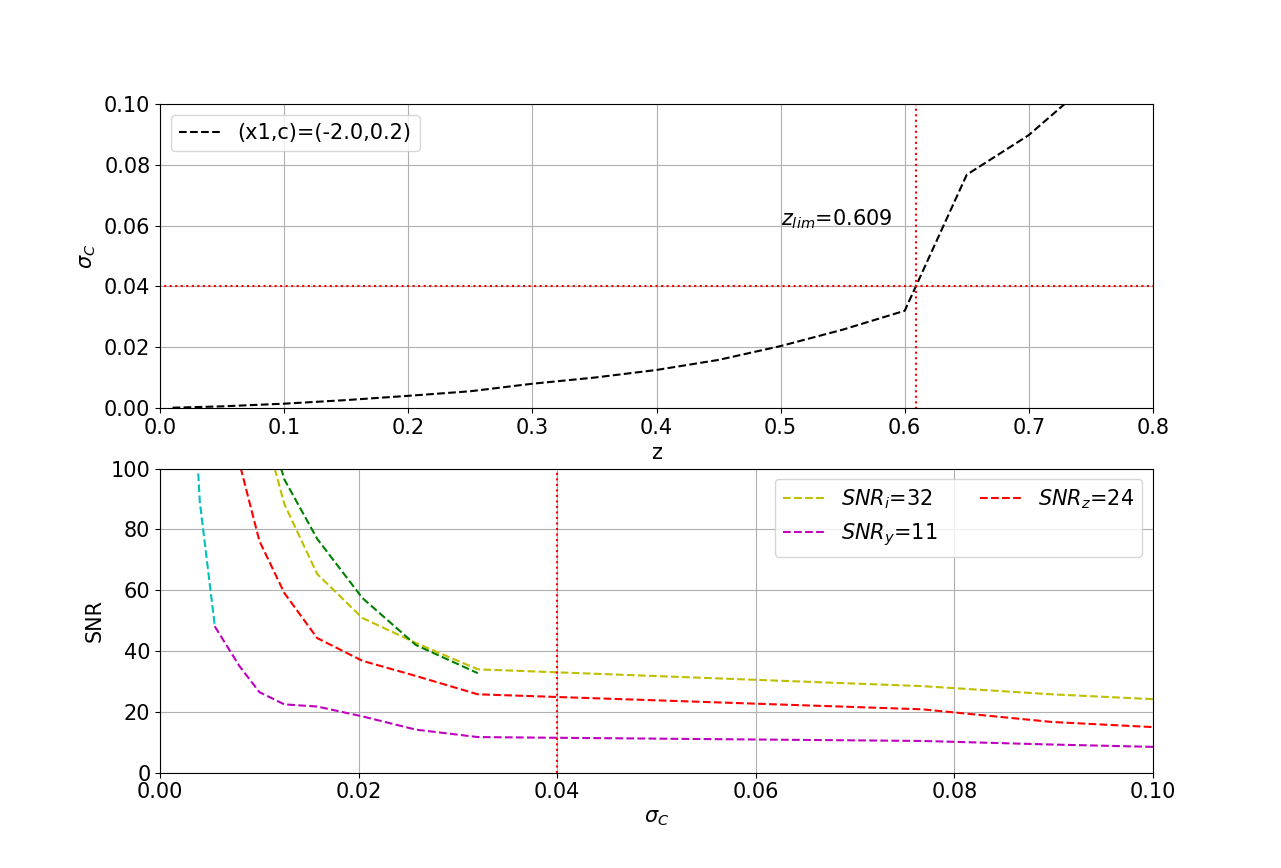
\includegraphics[width=0.9\textwidth]{sigmaC_z.png}
 \caption{Color error \sigc~as a function of redshift (top) and signal-to-noise ratio per band \snrb~as a function of \sigc~(bottom) for a faint type Ia supernova.}\label{fig:sigc_z}
\end{center}
\end{figure}


\section{LSST Deep Drilling program design constraints}
\label{sec:design}

Up to approximately 10\% of LSST observing time will be dedicated to other programs, including intensive observation of a set of Deep Drilling Fields. 

\begin{itemize}
\item number of fields: the location of four DD fields (\cosmos,\elais,\xmm,\cdfs) are already fixed (Tab. \ref{tab:locddf}). Two could be added in the south region (\adfa,\adfb) to ensure a synergy with \euclid~and \wfirst~surveys, at the begining and at the end of the LSST survey, respectively. 
\item season length: the number of exploding supernovae is proportional to the season duration. Season lengths of at least 6 months are required to maximize the size of the sample of observed type Ia supernovae.
\item cadence: observations every $\sim$3 days would lead to an adequate sampling of the light curves. 
\item DD budget: it is expected that 5-6$\%$ of the total number of LSST visits will be alloted to the DD program and shared among science topics interested by DD observations (such as AGN, supernovae, ...).  This limited budget is related to the total number of visits per observing night through the relation:
  \begin{eqnarray}
  DD_{budget} &=& N_{visits}^{DD}/N_{visits}^{tot} \\
  N_{visits}^{DD} &=& \sum_{i=1}^{N_{fields}} \sum_{ j=1}^{N_{season}^i} N_{visits,night}^{ij}\times SL^{ij}\times 30/Cad^{ij} 
  \end{eqnarray}
where $N_{fields}$ is the number of DD fields, $N_{season}$ the number of season of observations per field, $SL$ the season length, $Cad$ the cadence of observations, and $N_{visits, night}$ the total number of visits per observation night. $N_{visits,night}$ has been estimated for a cadence of 3 days, season lengths of 6 months, and $N_{visits}^{tot$}$ = (Tab. \ref{tab:ddbudget}). $N_{visits,night}$ largely depends on the observing strategy:   
  
 \end{itemize}

\begin{table}[!htbp]
  \caption{Location of the DD fields considered in this study.}\label{tab:locddf}
  \begin{center}
    \begin{tabular}{c|c|c}
      \hline
      \hline
      Field & Central RA & Central Dec\\ 
      Name & (J2000)  & (J2000)\\
      \hline
     \elais & 00:37:48 & −44:01:30 \\
     \xmm & 02:22:18 &  −04:49:00 \\
     \cdfs & 03:31:55 & −28:07:00 \\
     \cosmos &10:00:26 & +02:14:01 \\
     \hline 
     \adfa & 04:51:00& −52:55:00 \\
     \adfb & 04:35:00 & −54:40:00 \\
      \hline
      \hline
      \end{tabular}
  \end{center}
\end{table}

\begin{table}[!htbp]
  \caption{Total number of visits per night of observations for two number of fields (5 and 6) and two budgets (6\% and 10\%). The first (second) number correspond to 10 (2) seasons of observation per field. }\label{tab:ddbudget}
  \begin{center}
    \begin{tabular}{c|c|c}
      \hline
      \hline
      \diagbox[innerwidth=3.cm,innerleftsep=-1.cm,height=3\line]{$DD_{budget}$}{$N_{fields}$} & 5 & 6\\
      \hline
      6\% & 48/239& 40/199\\
      10\% & 80/398& 66/331 \\
      \hline
    \end{tabular}
  \end{center}
\end{table}



% ----------------------------------------------------------------------

%\section{Lessons from recent simulations}
%\label{sec:simu}


% ----------------------------------------------------------------------

\section{Optimization of the LSST Deep Drilling  program}
\label{sec:optimization}
\subsection{Optimization method}
\subsection{Results}

% ----------------------------------------------------------------------


\section{Proposal for new DD-minisurvey scenario}
\label{sec:proposal}

% ----------------------------------------------------------------------

\section{Discussion}
\label{sec:discussion}



% ----------------------------------------------------------------------

\section{Conclusion}
\label{sec:conclusion}



% ----------------------------------------------------------------------

\subsection*{Acknowledgments}

%%% Here is where you should add your specific acknowledgments, remembering that some standard thanks will be added via the \code{desc-tex/ack/*.tex} and \code{contributions.tex} files.

%This paper has undergone internal review in the LSST Dark Energy Science Collaboration. % REQUIRED if true

Author contributions are listed below. \\
Ph.~Gris: conceptualization,software,analysis,writing \\
N.~Regnault: conceptualization,writing \\
 % Standard papers only: author contribution statements. For examples, see http://blogs.nature.com/nautilus/2007/11/post_12.html

% This work used TBD kindly provided by Not-A-DESC Member and benefitted from comments by Another Non-DESC person.

% Standard papers only: A.B.C. acknowledges support from grant 1234 from ...

\input{desc-tex/ack/standard} % also available: key standard_short

% This work used some telescope which is operated/funded by some agency or consortium or foundation ...

% We acknowledge the use of An-External-Tool-like-NED-or-ADS.

%{\it Facilities:} \facility{LSST}

% Include both collaboration papers and external citations:
\bibliography{main,lsstdesc}

\end{document}

% ======================================================================
